\documentclass[main]{subfiles}


\title[AutoML: NAS]{Neural Architecture Search}
\subtitle{How to define Neural Architecture Search?}
\author[Jovita Lukasik]{Jovita Lukasik}
\date{}

\titlebackground*{images/AutoML_HPO_2_2}

%\institute{}
%\date{}

\begin{document}
	
	\maketitle


\begin{frame}{Definition of Neural Architecture Search}
\begin{center}
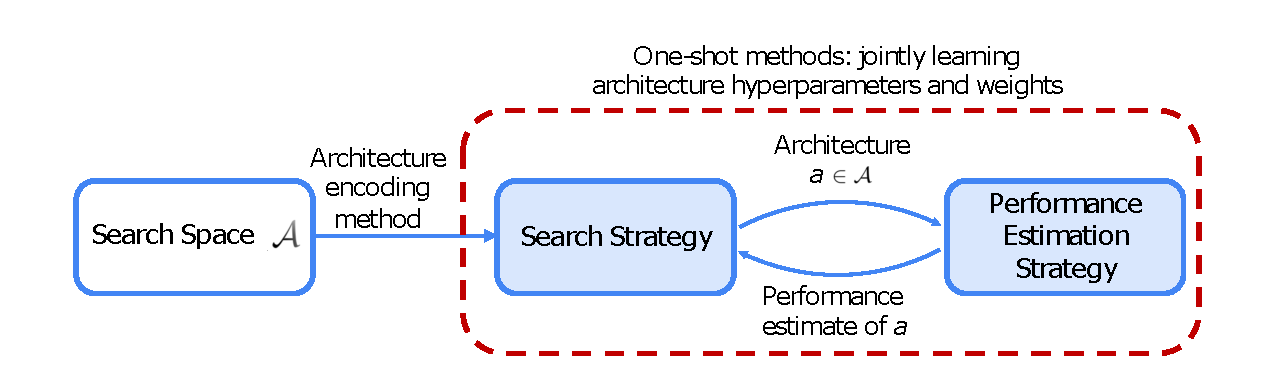
\includegraphics[height=3cm]{images/white_2023_nas_overview.pdf}
\captionof{figure}{Overview of neural architecture search ~\liturl{White et al. 2023}{https://arxiv.org/pdf/2301.08727.pdf}}
\end{center}
\begin{itemize}
    \item Different NAS components
        \begin{enumerate}
            \item Search Space
            \item Search strategy
            \item Performance estimation strategy
        \end{enumerate}
\end{itemize}
Question: Which component still needs the most human expert knowledge?
\end{frame}

\begin{frame}{Frame Title}

\begin{amsdefi}[\textbf{Neural Architecture Search}]\label{Def:NAS}
Given a search space $\mathcal{A}$, a dataset $D$, a training pipeline $P$ and a predefined time budget $T$. 
In Neural Architecture Search (NAS) the goal is to find an architecture $a \in \mathcal{A}$ with the highest validation accuracy when trained on $D$ with the training pipeline $P$ within the time budget $T$. 
This can be approached by approximately solve the following within $T$:
\begin{align}
  \begin{split}
  & \min_{a \in \mathcal{A}} \mathcal{L}_{\mathrm{val}}(w^*(a),a) \\
  &\mathrm{s.t.}~ w^*(a) = \underset{w}{\mathrm{argmin}} \mathcal{L}_{\mathrm{train}} (w,a),
  \end{split}
\end{align}
with $\mathcal{L}_{\mathrm{val}}$ and $\mathcal{L}_{\mathrm{train}}$ being the validation and training loss on data $D$, $w$ denotes the trained architecture weights. 
\end{amsdefi}
    
\end{frame}
%----------------------------------------------------------------------
\begin{frame}{Summary} 

Most important insights from this video:

\begin{enumerate}
    \item ???
    \item ???
    \item ???
\end{enumerate}


\end{frame}



\end{document}
